% arara: xelatex
% arara: xelatex

\documentclass{beamer}
\usepackage{menukeys}
\usepackage{multicol}
\usepackage{mwe}
\usepackage{style}
\usepackage{listings}
\usepackage{smcm-cosc-listings}
\usetikzlibrary{fit,shapes,arrows,arrows.meta}
\usepackage{fontspec}
\setmonofont{Courier}
\setlength\labelsep{1.5ex}
\setlength\fboxsep{1ex}
\usepackage{dirtree}

\usepackage[absolute,overlay]{textpos}

\usepackage{tikz}
\usetikzlibrary{fadings}

\newlength\mylongedgegradlen
\newlength\myshortedgegradlen
\newlength\mylongedgemargin
\newlength\myshortedgemargin
\setlength\mylongedgegradlen  { 2 in}
\setlength\myshortedgegradlen { 2 in}
\setlength\mylongedgemargin   {30 mm}
\setlength\myshortedgemargin  {30 mm}

\usetikzlibrary{calc}

\begin{document}
\begin{frame}[fragile,t]
  \maketitle
  \vspace{1in}
  \begin{columns}[t]
    \begin{column}{.45\textwidth}
      \begin{block}{Abstract}
        In computer science,
            a self-stabilizing algorithm is
            a fault-tolerant problem-solving process that,
            when applied repeatedly to a system,
            will coerce the system into a ‘correct state’.
        Given their parallel nature,
            algorithms of this class are sometimes more difficult
            to create and prove correct than
            more traditional, procedural algorithms.
        To aid in further research,
            \st provides an extensible utility for
            the representation, creation, and evaluation
            of self-stabilizing algorithms.
      \end{block}

      \begin{block}{Example \Dash Maximal Independent Set}
        \begin{minipage}[b]{4in}
          \begin{enumerate}
            \large
          \item[1]
            \begin{tikzpicture}[baseline=1in,scale=1.5]
              \node[graph vertex, marked] (1) at (0 , 3) {$v_1$};
              \node[graph vertex,       ] (2) at (0 , 6) {$v_2$};
              \node[graph vertex,       ] (3) at (3 , 3) {$v_3$};
              \node[graph vertex, marked] (4) at (3 , 6) {$v_4$};
              \node[graph vertex,       ] (5) at (5 , 8) {$v_5$};
              
              \graph {
                (1) -- (3) -- (4) -- (2) --[bend left] (5),
                (1) -- (2),
                (1) -- (4),
                (3) --[bend right] (5)
              };
            \end{tikzpicture}
          \item[2]
            \begin{tikzpicture}[baseline=1in,scale=1.5]
              \node[graph vertex, marked] (1) at (0 , 3) {$v_1$};
              \node[graph vertex,       ] (2) at (0 , 6) {$v_2$};
              \node[graph vertex,       ] (3) at (3 , 3) {$v_3$};
              \node[graph vertex, marked] (4) at (3 , 6) {$v_4$};
              \node[graph vertex, marked] (5) at (5 , 8) {$v_5$};
              
              \graph {
                (1) -- (3) -- (4) -- (2) --[bend left] (5),
                (1) -- (2),
                (1) -- (4),
                (3) --[bend right] (5)
              };
            \end{tikzpicture}
          \item[3]
            \begin{tikzpicture}[baseline=1in,scale=1.5]
              \node[graph vertex, marked] (1) at (0 , 3) {$v_1$};
              \node[graph vertex,       ] (2) at (0 , 6) {$v_2$};
              \node[graph vertex,       ] (3) at (3 , 3) {$v_3$};
              \node[graph vertex,       ] (4) at (3 , 6) {$v_4$};
              \node[graph vertex, marked] (5) at (5 , 8) {$v_5$};
              
              \graph {
                (1) -- (3) -- (4) -- (2) --[bend left] (5),
                (1) -- (2),
                (1) -- (4),
                (3) --[bend right] (5)
              };
            \end{tikzpicture}
          \end{enumerate}
        \end{minipage}
        \hfill
        \begin{minipage}[b]{9in}
          \newcommand\fOf[1]{f\,(\mkern -1mu #1)}
          \vfill
          \centerline{\IndSet}
          \vspace{2ex}
\begin{lstlisting}[language=ssa,frame=lines]
local $f$

privilege ENTER
  if $\fOf{v} = 0 \land \ForAll{n \in \OpenNeighborhood{\mkern -1mu v \mkern .75mu}}{\fOf{n} = 0}$
  then:
    $\fOf{v} = 1$

privilege LEAVE
  if $\fOf{v} = 1 \land \Exists{\,n \in \OpenNeighborhood{\mkern -1mu v \mkern .75mu}}{\fOf{n} = 1}$
  then:
    $\fOf{v} = 0$
\end{lstlisting}
          \vspace{.5in}
          The algorithm for maximal independent set consists of two possible privileges:
          \bigskip
          \begin{description}[\texttt{ENTER}]
          \item[\texttt{ENTER}] Not marked and \emph{no} neighbor marked
          \item[\texttt{LEAVE}] Marked and \emph{any} neighbor marked
          \end{description}
          \bigskip
          If either statement is true for any node $v_i$,
            that privilege is `present' on $v_i$
            and $v_i$ could move.
          Under a central daemon,
            a privileged node is arbitrarily chosen to make its move,
          When this move completes,
            all privileges are re-evaluated
            and the process repeats.
          \vfill
          ~
        \end{minipage}
        \vspace*{-2ex}
      \end{block}

      \begin{block}{Definition}
        Self-stabilizing algorithms work with sparse, connected graphs of state machines where
          the algorithm is defined either in a central daemon or within each state machine:
        \begin{description}[algorithmMMMM]
        \item[predicate] $\Function[f]{v, N(\mkern -1mu v\mkern .75mu)}{\SetBoolean}$
        \item[move] new state for $v$
        \item[rule] $\Function[R]{P}{M}$
        \item[algorithm] $\Set{\QuickSequence{R}}$
        \end{description}
        \begin{center}
        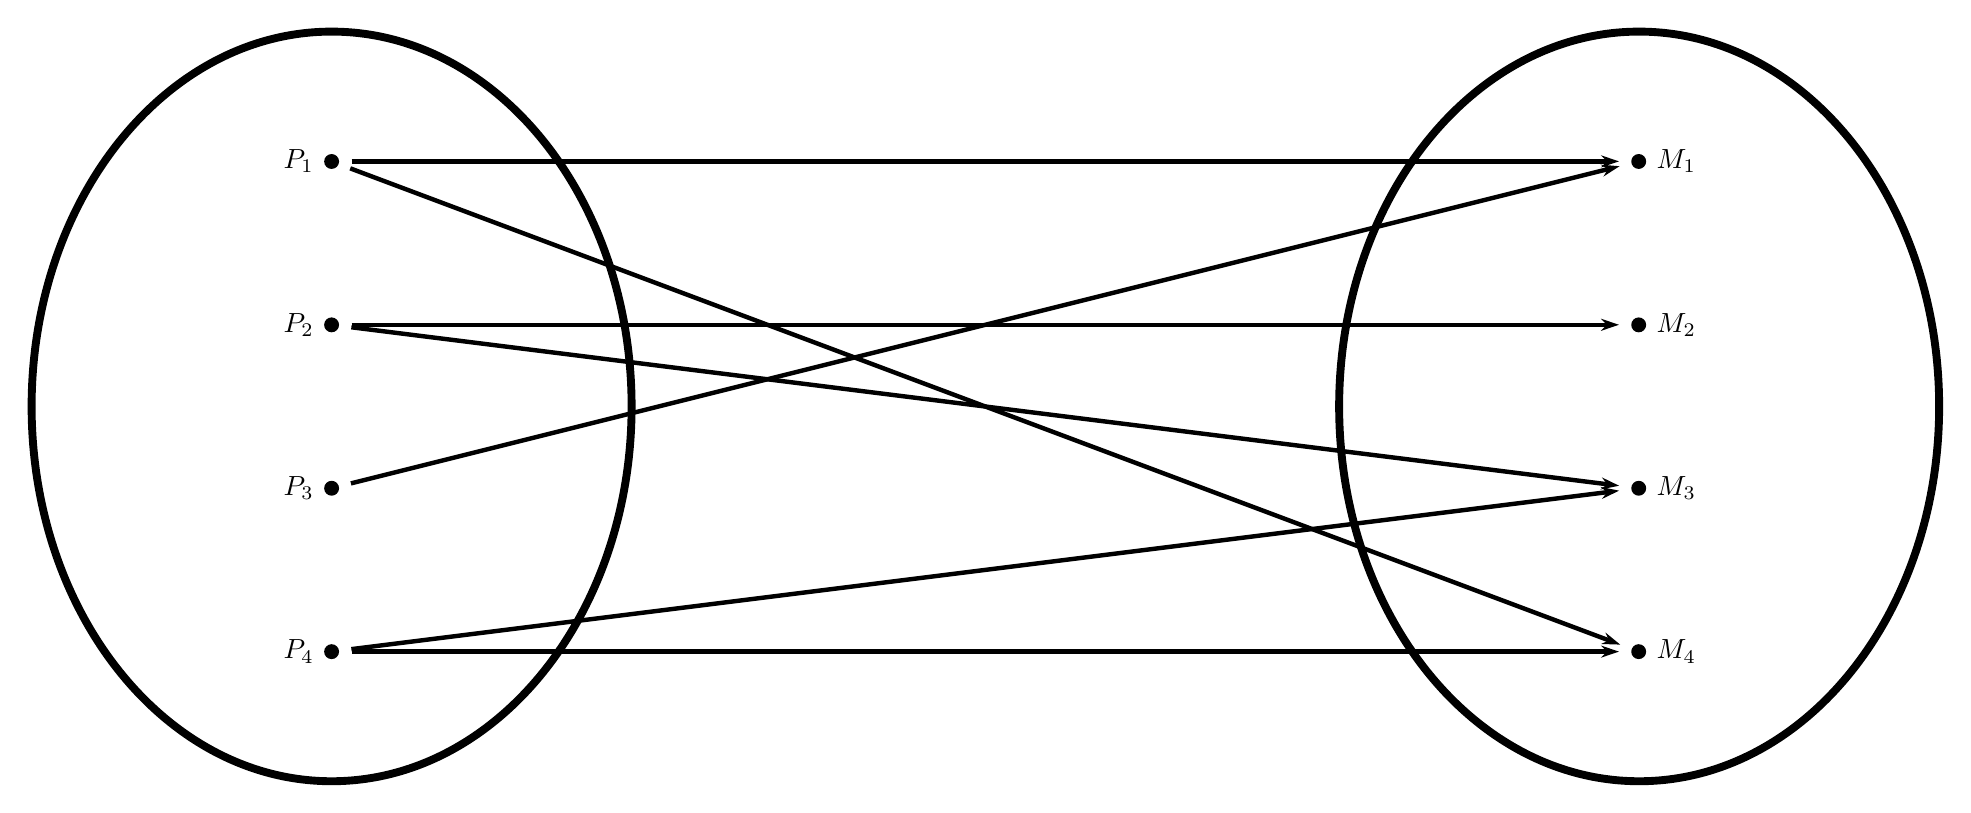
\begin{tikzpicture}[scale=2.075,
          >=stealth,
          bullet/.style={
            fill=black,
            circle,
            minimum width=1.25ex,
            inner sep=1pt
          },
          projection/.style={
            -{Stealth[width=1ex,length=1.5ex]},
            ultra thick,
            shorten <=1ex,
            shorten >=1ex,
          },
          every fit/.style={
            ellipse,
            line width=1mm,
            draw,
            inner sep=1ex
          }
          ]
          \foreach \y/\l in {1/4,2/3,3/2,4/1} {
            \node[bullet,label=left:$P_\l$] (p\l) at (0,\y) {};
            \node[bullet,label=right:$M_\l$] (m\l) at (8,\y) {};
          }
          
          \node[draw,fit=(p1) (p2) (p3) (p4),minimum width=3in] {} ;
          \node[draw,fit=(m1) (m2) (m3) (m4),minimum width=3in] {} ;
          
          \draw[projection] (p1) -- (m1);
          \draw[projection] (p1) -- (m4);
          \draw[projection] (p2) -- (m2);
          \draw[projection] (p2) -- (m3);
          \draw[projection] (p3) -- (m1);
          \draw[projection] (p4) -- (m4);
          \draw[projection] (p4) -- (m3);
        \end{tikzpicture}
        \end{center}
        \vspace{-.03in}
      \end{block}
      \begin{block}{Further Work}
        \begin{multicols}{2}
          \begin{itemize}
          \item integrated graph manipulation
          \item integrated test visualization
          \item integrated test cases
          \item alternative run modes
          \item parallelization of execution
          \item API for passive integration
          \end{itemize}
        \end{multicols}
        \vspace{0.01in}
      \end{block}
    \end{column}
    \begin{column}{.45\textwidth}
      \begin{block}{The Bundle Format}
        To store these algorithms on disk, \st uses a two-fold approach:
        \begin{itemize}
        \item A series of YAML documents is maintained to provide
          metadata for the basic entities as well as depict the
          relationships between those entities
        \item Basic components (predicates\slash moves) are maintained
          without repetition in a predetermined, configurable
          directory structure within \directory{%
            {$\langle${\itshape bundle}$\rangle$}\kern-4pt.ssax}
        \end{itemize}

        \begin{minipage}{\linewidth}
          \hfill
          \begin{minipage}{5in}
\begin{lstlisting}[language=yaml,basicstyle=\ttfamily\YAMLkeystyle\large]
--- !Move
name: mark
filename: mark.py
--- !Move
name: unmark
filename: unmark.py
--- !Predicate
name: node should mark
filename: enter.py
--- !Predicate
name: node should unmark
filename: leave.py
--- !Algorithm
name: Independent Set
rules:
  - !Rule
    predicate: enter
    moves: [ mark ]
  - !Rule
    predicate: leave
    moves: [ unmark ]
\end{lstlisting}
          \end{minipage}
          \hfill
          \begin{minipage}{5in}
            \raggedright
            Under this structure, \IndSet would look similar to this
            (with much more metadata)

            \vspace{2in}

            \large
            \linespread{1.1}

            \dirtree{%
              .1 ind-set.ssax/.
              .2 bundle.yaml.
              .2 predicates/.
              .3 enter.py.
              .3 leave.py.
              .2 moves/.
              .3 mark.py.
              .3 unmark.py.
            }
            
          \end{minipage}
          \hfill
          ~
        \end{minipage}

        with all necessary files, such as \directory{ind-set.ssax/predicates/enter.py}, included:
        \vspace{.3in}
\begin{lstlisting}[language=Python,stringstyle=\color{green!50!black},keywordstyle=\color{blue},basicstyle=\ttfamily\large]
  marked = v['marked']
  neighbor_marked = any(map(lambda n: n['marked'], N))
  return not (marked or neighbor_marked)
\end{lstlisting}
\vspace*{-1ex}
      \end{block}
      
      \begin{block}{Interface}

        \setlength\fboxsep{0pt}
        \setlength\fboxrule{.1ex}
        \vspace*{-.75in}
        \begin{center}
          \fcolorbox{black!50}{black!50}{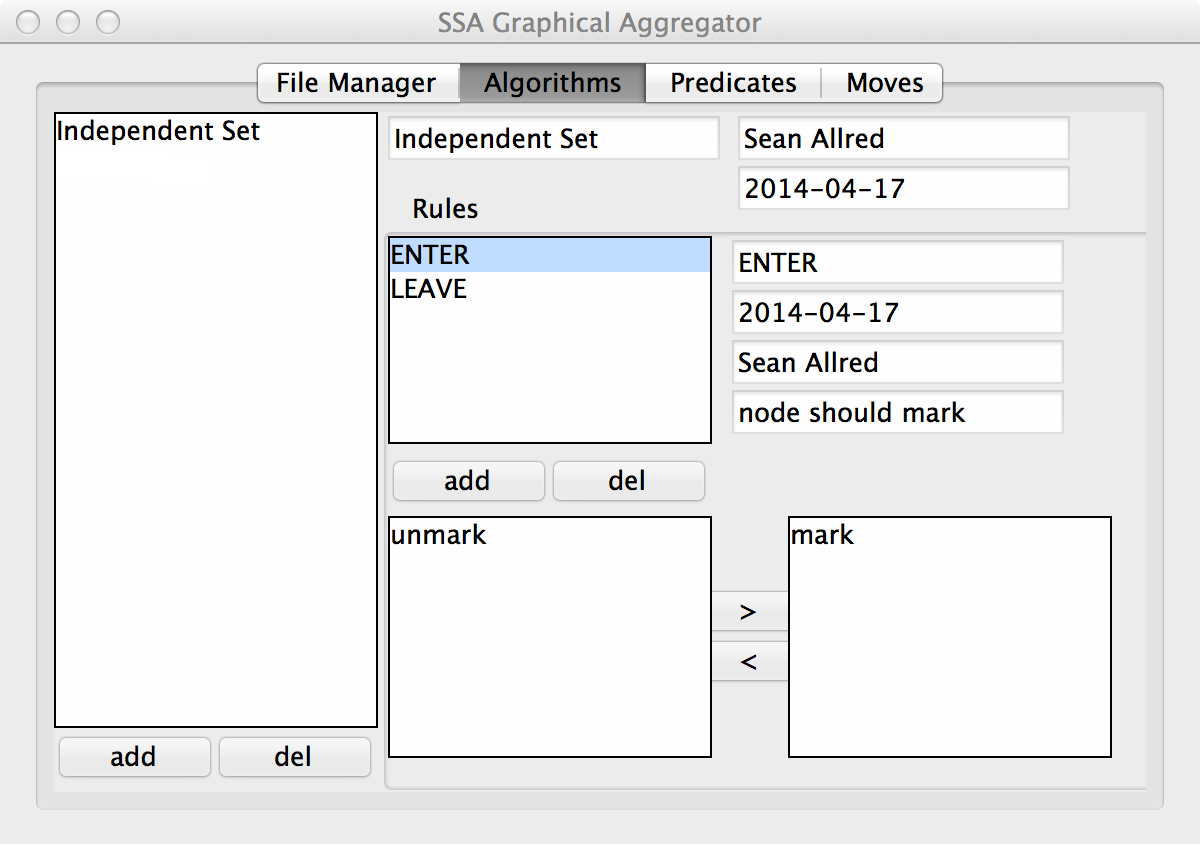
\includegraphics[width=\linewidth]{../figs/4}}
        \end{center}
        \fcolorbox{black!50}{black!50}{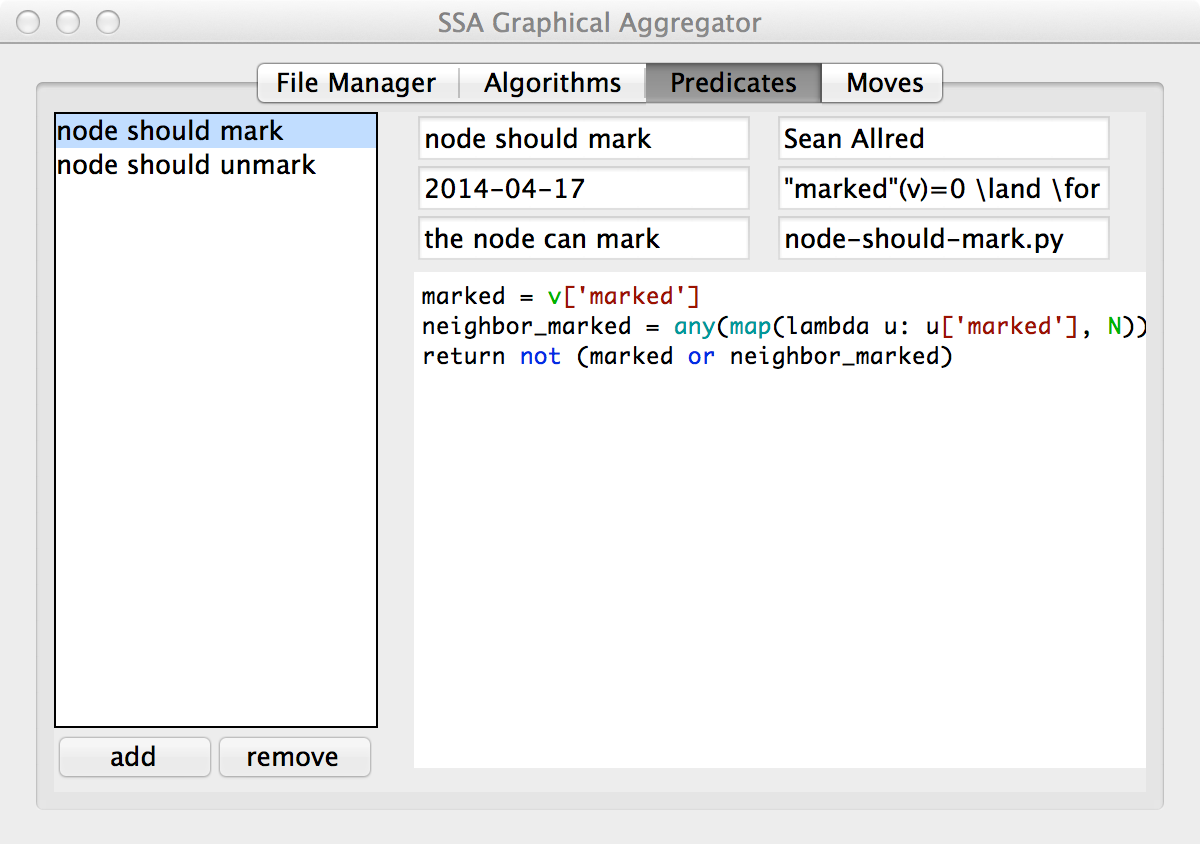
\includegraphics[width=.49\linewidth]{../figs/2}}
        \begin{minipage}[b]{.49\linewidth}
          \raggedleft

          As the algorithm runs, a log is kept of changes to the
          graph.  When the process completes, these changes are
          returned as a custom-made \texttt{AnimatedGraph} object that
          can traverse the entire history of the graph frame-by-frame.

          \vspace*{2ex}
        \end{minipage}%
        \vspace*{-1ex}
      \end{block}
    \end{column}
  \end{columns}
\end{frame}
\end{document}

%%% Local Variables:
%%% mode: latex
%%% TeX-master: t
%%% TeX-PDF-mode: t
%%% TeX-command-default: "arara"
%%% truncate-lines: nil
%%% TeX-engine: xetex
%%% End:
